\documentclass[hyperref={colorlinks=false},handout,10pt]{beamer}
\usetheme{Singapore} % Berlin
\usecolortheme{lily} %{wolverine} %lily
\usefonttheme[onlymath]{serif} % What does this do? 

\newcommand{\mygreen}{\color{green!50!black}}
\newcommand{\myblue}{\color{blue}}
\newcommand{\myred}{\color{red}}
\xdefinecolor{titlecolor}{rgb}{.855,.647,.125}
\setbeamercolor{frametitle}{fg=titlecolor}
\setbeamerfont{frametitle}{series=\bfseries}
%\setbeamerfont{headline}{size=\fontsize{9}{1}}
\setbeamercolor{math text}{fg=green!50!black} % Why is the math text greeen?? 
\setbeamercolor{normal text in math text}{parent=math text}

\setbeamertemplate{navigation symbols}{} %gets rid of navigation symbols
%\setbeamertemplate{mini frames}{}
\setbeamertemplate{footline}[frame number]
\beamertemplateshadingbackground{blue!5}{yellow!10}


\usepackage{graphicx}
%\usepackage{tikz}
%\usepackage{handoutWithNotes}
%\pgfpagesuselayout{4 on 1 with notes}[a4paper,border shrink=2mm]

\usepackage{pgfpages}
\pgfpagesuselayout{4 on 1}[a4paper, border shrink=5mm, landscape]

\newlength{\wideitemsep}
\setlength{\wideitemsep}{\itemsep}
\addtolength{\wideitemsep}{100pt}
\let\olditem\item
\renewcommand{\item}{\setlength{\itemsep}{0.5\baselineskip}\olditem}


\def\LaTeXs{\LaTeX\ }

%\usetikzlibrary{calc,fadings,decorations.pathreplacing,backgrounds}
%% helper macros
%\tikzset{variable/.default=}  
%\tikzset{%
%    add/.style args={#1 and #2}{ to path={%
%    ($(\tikztostart)!-#1!(\tikztotarget)$)--($(\tikztotarget)!-#2!(\tikztostart)$)%
%\tikztonodes},add/.default={.2 and .2}}
%}  

%\tikzset{%
%    >=latex,
%    inner sep=0pt,
%    outer sep=2pt,
%    mark coordinate/.style={inner sep=0pt,outer sep=0pt,minimum size=2pt,
%    fill=black,circle}%
%}

\usepackage{textcomp}
\usepackage{listings}
\lstset{
basicstyle=\footnotesize\ttfamily,
language=R,
upquote=true,
breakatwhitespace=true,
columns=fullflexible,
keepspaces,
%numbers=none,
tabsize=3,
frame=bottomline,
framextopmargin=50pt,
showstringspaces=false,
extendedchars=true
}

\usepackage{amsmath,amsthm,amssymb}


\usepackage{float}
\floatstyle{boxed} % What does this do? 
\usepackage{mathpazo}
\usepackage{movie15}
\usepackage{bm}
%\usepackage{comment} % What does this do? 
\usepackage{caption}
\usepackage{subcaption}
\captionsetup[subfigure]{labelformat=empty}
\captionsetup[figure]{labelformat=empty}
\graphicspath{{./images/}}


\title{{\color{blue} \LARGE 550.400: Mathematical Modeling and Consulting\newline} }

\subtitle{{\color{red} \large Lecture Notes} }

\author{ 
    {\bf{Instructor:}} \\ 
Dr.~N.~H.~Lee \\ 
    \vspace{5pt}
} 
\institute{JHU AMS 2012 FALL}

\date{\mygreen Last Compiled on \today} 


\begin{document}

\begin{frame}[plain]
  \titlepage
\end{frame}

Hello

\begin{figure}
    \begin{center}
        \includegraphics[width=\textwidth]{somefigurefile.png}
    \end{center}
    \caption{This is a sample}
    \label{fig:sample}
\end{figure}

\begin{env}
    <++>
\end{env}

\begin{frame}
    \frametitle{Hello World}
    Hello World.
\end{frame}


\begin{frame}%[shrink]
  \frametitle{Outline}
  \tableofcontents
\end{frame}

\section{FAQ} 

\begin{frame}
    \frametitle{Adobe Connect}
    \begin{center}
        \Large
        \href{https://connect.johnshopkins.edu/meeting550400/}{https://connect.johnshopkins.edu/meeting550400/}
\end{center}
\end{frame}

\begin{frame}
    \frametitle{Announcement}
    \begin{itemize}
        \item HW \emph{SET} $1$ due on Monday Oct 8
        \item Include your drawing in HW SET $1$ as a figure
        \item Marked Work Statement is returned on Monday Oct 8
        \item Check the blackboard frequently for updates
        \item Ask non-sensitive questions on Blackboard Discussion Forum FAQ
    \end{itemize}
\end{frame}

%\begin{frame}
%    \frametitle{Quiz}
%    \begin{itemize}
%        \item Create a github repository with your favorite quote as a text
%            file \texttt{main.txt},
%        \item Post your github location in the designated Discussion forum 
%            by creating a thread just for yourself,
%        \item Collect all of your classmates' quote only using git,
%        \item You should have at least four commits, each adding new materials
%            to the file \texttt{main.txt},
%        \item You have twenty minutes to complete the quiz.
%    \end{itemize}
%\end{frame}

\begin{frame}
    \frametitle{Git FAQ}
    \begin{center}
        \href{http://gitref.org/index.html}{http://gitref.org/index.html}
    \end{center}
\end{frame}

\begin{frame}
    \frametitle{Vim FAQ}
    In Vim, how do you
    \begin{itemize}
        \item start, save, quit Vim? 
        \item show numbers on the side?
        \item change the color theme?
        \item move around?
        \item spell check?
        \item find particular words?
        \item save typing while coding these \LaTeX\ commands?
        \item install plugins?
    \end{itemize}
\end{frame}

\begin{frame}
    \frametitle{Vim FAQ}
    \begin{block}
        {Vim is a \emph{highly customizable} text editor}
    \vskip0.1in
    \begin{enumerate}
        \item \LaTeX, R, C/C++, Java, Python, Git and etc.
        \item Regular expression, syntax coloring, auto-completion
        \item \texttt{<ESC>}-mode
        \begin{itemize}
            \item \texttt{:}-mode, aka., the last line mode
            \item \texttt{i}-mode, aka., the insert mode
        \end{itemize}
    \end{enumerate}
    \end{block}
\end{frame}

\begin{frame}
    \frametitle{Vim FAQ}
    \begin{itemize}
        \item Download \& Install GVim or MacVim
        \item Download \& Install tetris.vim
        \item Download \& Install minibufexpl.vim
        \item Download \& Install Gundo 
        \item Download \& Install Vim-LaTeX
    \end{itemize}
\end{frame}

\begin{frame}
    \frametitle{Vim FAQ}
    \begin{figure}
        \begin{center}
            \includegraphics[width=\textwidth]{images/vi-vim-tutorial-1.png}
        \end{center}
    \end{figure}
\end{frame}

\begin{frame}[fragile]
    \frametitle{\LaTeXs FAQ}
    \begin{block}{How do you add a figure in \LaTeXs?}
    \begin{lstlisting}
\begin{figure}
    \caption{<+caption text+>}
    \begin{center}
        \includegraphics[width=<+number+>\textwidth]{<+filename+>}
    \end{center}
\end{figure}
    \end{lstlisting}
     Here, \verb$<+...+>$ denotes a thing that you need to fill in.
    \end{block}
    \begin{block}{But you will need this in the preamble part of your \LaTeX:}
    \begin{lstlisting}
\usepackage{graphicx} 
    \end{lstlisting}
    To save yourself from unnecessary glitches, insert \texttt{png},
    \texttt{jpeg}, \texttt{pdf} files only.
    \end{block}
\end{frame}

\begin{frame}
    \frametitle{Cross Sectional Study Vs.\ Longitudinal Study}
    \begin{figure}
        \centering
            \href{http://www.wired.com/magazine/2010/11/ff_311_new_york/all/}{ 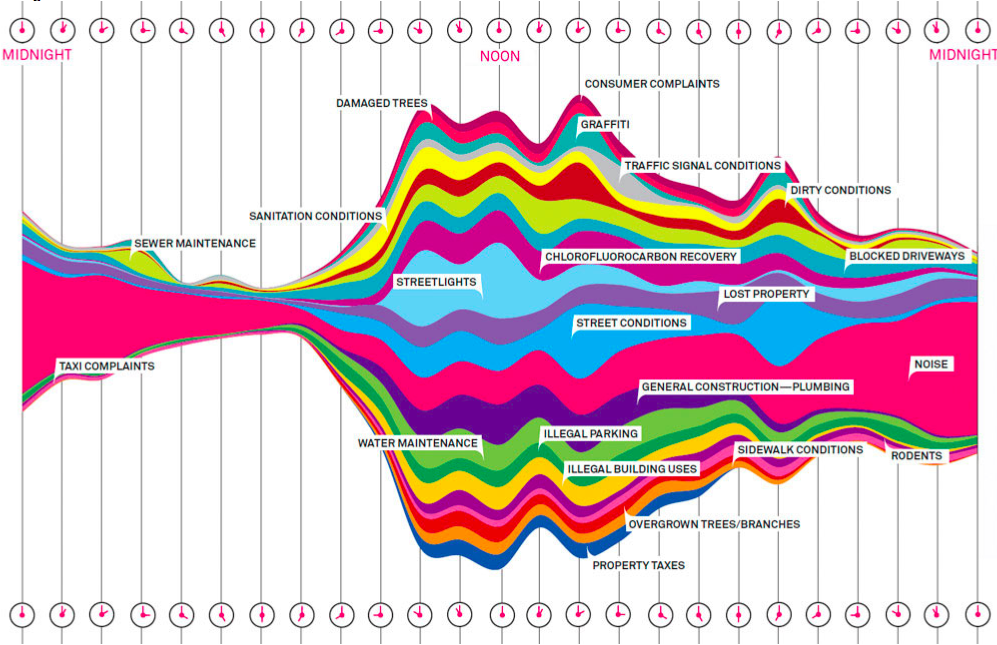
\includegraphics[scale=0.3]{images/311callvolume.png}}
            \caption{There were 34,522 complaints called in to 311 between September 8 and September 15, 2010. Here are the most common, plotted by time of day.}
    \end{figure}
\end{frame}

\begin{frame}
    \frametitle{Can Riots Be Predicted?}
    \begin{figure}
        \caption{A Tunisian protester holds a baguette while taking to riot police in January 2011}
        \begin{center}
            \href{http://www.npr.org/blogs/thesalt/2012/09/20/161501075/high-food-prices-forcast-more-global-riots-ahead-researchers-say}{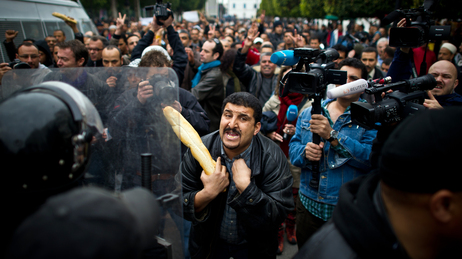
\includegraphics[width=\textwidth]{images/food_riot.jpg}}
        \end{center}  
    \end{figure}
\end{frame}

%\begin{frame}
%    \frametitle{Commit? Add? What is the difference?}
%    \begin{block}{An imperfect analogy}
%        \begin{itemize}
%            \item Just like doing your HW with many questions
%            \item For each question, first you do some work
%            \item \texttt{git add} is like you being satisfied with your current
%                version of your answer
%            \item \texttt{git commit} is like you transcribing your solution to your
%                paper that you will actually submit
%            \item \texttt{git push} is like submitting your solution to the
%                instructor so that they can see
%        \end{itemize}
%    \end{block}
%\end{frame}



%\section{Git} 
%\begin{frame}[allowframebreaks,fragile]
%    \frametitle{Class Exercise}
%    \begin{block}{Exercise 1}
%    \begin{figure}
%        \caption{\Large This is called a \emph{commit} graph}
%        \begin{center}
%            \includegraphics[width=\textwidth]{images/gitmergehistory.png}
%        \end{center}
%    \end{figure}
%    \end{block}
%    \vskip0.5in
%    
%    \begin{block}{Create a git folder with the following history}
%         \begin{itemize}
%             \item Each node's label signifies the commit 
%             \item The folder contains only one single file \texttt{main.txt}
%                 throughout the history
%             \item Keep ``the story'' simple
%             \item Push it to your github (remote) repository
%         \end{itemize}
%    \end{block}
%
%    \begin{block}{Exercise 2}
%        Collect all 8 stanzas of the ``Elephant'' poem from the course 
%        github remote repositories and then push the resulting 
%        one to \emph{your} github repository.
%    \end{block}
%    You will need the following addresses:
%    \begin{lstlisting}
%git://github.com/nhlee/550400.stanza1.git 
%git://github.com/nhlee/550400.stanza2.git 
%git://github.com/nhlee/550400.stanza3.git 
%git://github.com/nhlee/550400.stanza4.git 
%git://github.com/nhlee/550400.stanza5.git 
%git://github.com/nhlee/550400.stanza6.git 
%git://github.com/nhlee/550400.stanza7.git 
%git://github.com/nhlee/550400.stanza8.git 
%    \end{lstlisting}
%\end{frame}


%\begin{frame}[allowframebreaks,fragile]
%    \frametitle{Adv. Git Method for Off-Line Teamwork}
%    \begin{figure}
%        \begin{center}
%            \includegraphics[width=0.8\textwidth]{images/gitmergeexample.png}
%        \end{center}
%    \end{figure}
%    \begin{lstlisting}
%git branch alice 
%git checkout alice
%git remote add altorigin git://git.com/do/not/copy/and/paste/this
%git push origin alice
%git branch -D alice
%    \end{lstlisting}
%
%    \begin{lstlisting}
%git format-patch master~2..master
%    \end{lstlisting}
%    \begin{figure}
%        \begin{center}
%            \includegraphics[width=0.7\textwidth]{images/gitformatpatch.png}
%        \end{center}
%    \end{figure}
%\end{frame}


%\section{\LaTeX}
%\begin{frame}[allowframebreaks,fragile]
%    \frametitle{Intro.\ to work-statement template}
%    
%    
%\end{frame}

\begin{frame}[fragile]
    \frametitle{\LaTeXs FAQ}
    \begin{block}{How can I code a beamer?} 
\begin{lstlisting}
\documentclass[hyperref={colorlinks=false},handout,10pt]{beamer}
\usetheme{Singapore}
\usecolortheme{lily}
\usefonttheme[onlymath]{serif} % What does this do? 
\end{lstlisting}    
    OR
\begin{lstlisting}
\documentclass[hyperref={colorlinks=false},handout,10pt]{beamer}
\usetheme{Berlin}
\usecolortheme{wolverine}
\usefonttheme[onlymath]{serif} % What does this do? 
\end{lstlisting}    
\end{block}
    For a more complete array of themes, go to: 
    \begin{center}
        \href{http://www.hartwork.org/beamer-theme-matrix/}{{http://www.hartwork.org/beamer-theme-matrix/}}
    \end{center}
\end{frame}

\begin{frame}[fragile]
    \frametitle{\LaTeXs FAQ}
    \begin{block}{How can I code a beamer?: a single side with no block}
    \begin{lstlisting}
\begin{document}
        \begin{frame} # one frame per one slide
            \frametitle{hello world} # optional but you want one
                \begin{itemize}
                    \item apple
                    \item orange
                \end{itemize}
        \end{frame}
\end{document}
    \end{lstlisting}
    \end{block}
    \begin{block}{How can I code a beamer?: a single side with one block}
    \begin{lstlisting}
\begin{document}
        \begin{frame} # one frame per one slide
            \frametitle{hello world} # optional but you want one
                \begin{block}{hey world}
                    Bob!
                \end{block}
        \end{frame}
\end{document}
    \end{lstlisting}
    \end{block}
\end{frame}


\begin{frame}[fragile]
    \frametitle{\LaTeXs FAQ}
    \begin{block}{How can I code a beamer?: two slides}
    \begin{lstlisting}
\begin{document}
        \begin{frame} # one frame per one slide
            \frametitle{hello world} # optional but you want one
            \begin{itemize}
                \item apple
                \item orange
            \end{itemize}
        \end{frame}
        \begin{frame} # one frame per one slide
            \frametitle{hello world} # optional but you want one
                \begin{block}{hey world}
                    Bob!
                \end{block}
        \end{frame}
\end{document}
    \end{lstlisting}
    \end{block}
\end{frame}

\begin{frame}[fragile]
    \frametitle{\LaTeXs FAQ}
    \begin{block}{How can I code a beamer?: a single frame with two columns}
    \begin{lstlisting}
\begin{document}
        \begin{frame} # one frame per one slide
            \frametitle{hi world} # optional but you want one
            \begin{columns}
                \begin{column}{0.5\textwidth}
                    \begin{itemize}
                        \item Alice!
                    \end{itemize}
                \end{column}
                \begin{column}{0.5\textwidth}
                    \begin{block}{hey world}
                        Bob!
                    \end{block}
                \end{column}
            \end{columns} 
        \end{frame}
\end{document}
    \end{lstlisting}
    \end{block}
\end{frame}

\begin{frame}[fragile]
    \frametitle{\LaTeXs FAQ}
    \begin{block}{How can I code a beamer?: with a table of contents}
    \begin{lstlisting}
\begin{document}

    \begin{frame}
      \frametitle{Outline}
      \tableofcontents
    \end{frame}

    \section{Hello World}  # optional 
        \subsection{hello world} # optional 
            \begin{frame} # one frame per one slide
                \frametitle{hi world} # optional but you want one
            \end{frame}

    \section{Hello New World}
            \begin{frame} # one frame per one slide
                \frametitle{hi new world} # optional but you want one
            \end{frame}
\end{document}
    \end{lstlisting}
    \end{block}
\end{frame}

\begin{frame}[fragile]
    \frametitle{\LaTeX\ FAQ}
SO, how to put a code in the slide? and it looks like codes? 
\begin{columns}
    \begin{column}{0.5\textwidth}
    \begin{verbatim}
\begin{lstlisting}
require(tikzDevice)
x = rnorm(100)
plot.ts(x)
dev.off()
\end{lstlisting}
    \end{verbatim}
    \end{column}
    \begin{column}{0.5\textwidth}
\begin{lstlisting}
require(tikzDevice)
x = rnorm(100)
plot.ts(x)
dev.off()
\end{lstlisting}
    \end{column}
\end{columns} 
\end{frame}

\begin{frame}[fragile]
    \frametitle{\LaTeX\ FAQ}
But, this requires the following in the preamble portion 
of your tex file:
\begin{verbatim}
    \usepackage{listings}
    \lstset{
    basicstyle=\footnotesize\ttfamily,
    numbers=left,
    frame=bottomline,
    framextopmargin=50pt,
    }
\end{verbatim}
You will also need \texttt{fragile} option for your frame:
\begin{verbatim}
    \begin{frame}[fragile]
        \frametitle{hello world}
         \begin{lstlisting}
    x = rnorm(100)
         \end{lstlisting}
    \end{frame}
\end{verbatim}
\end{frame}

\begin{frame}
    \frametitle{\LaTeX\ FAQ}
Where to get more help:
\begin{center}
    \href{http://en.wikibooks.org/wiki/LaTeX/Presentations}{
    {http://en.wikibooks.org/wiki/LaTeX/Presentations}}
\end{center}
\end{frame}

%\section{R}


\begin{frame}[fragile]
    \frametitle{R FAQ}
    \begin{lstlisting}
for(itr in 1:8) {
    stanzaname = paste("stanza",itr,sep="")
    gitaddress = paste("git://github.com/nhlee/550400.",
                            stanzaname,".git",sep="")
    bashcommand = paste("git remote add ",
                            stanzaname," ",gitaddress,sep="")
    system(bashcommand)
}
    \end{lstlisting}
    \begin{itemize}
        \item \texttt{1:8} creates a vector that \ldots 
        \item \texttt{X = 1} assigns 1 to X 
        \item \texttt{X <- 1} also assigns 1 to X
        \item lots of things are done through function 
        \item \texttt{paste} and \texttt{system} are functions that \ldots 
        \item functions has none or more arguments 
        \item arguments are implicitly ordered but the order can be overridden
    \end{itemize}
\end{frame}

\begin{frame}[fragile]
    \frametitle{R FAQ}
    \begin{lstlisting}
system(`ls -ld .*')
system(`cat .Rprofile')
system(`cat .bashrc')
system(`cat .gitignore')
system(`cat .vimrc')
    \end{lstlisting}
    \begin{itemize}
        \item .xxx files are hidden
        \item ls -ld .* show the hidden files
        \item .Rprofile set up your R behavior
        \item .bashrc set up your bash behavior
        \item .gitignore set up your git behavior 
        \item .vimrc set up you vim behavior
        \item these files are equivalent to Preference part of your GUI
            software
    \end{itemize}
\end{frame}

\begin{frame}[fragile]
    \frametitle{R FAQ}
    {How to do software documentation (via R)}
     \begin{lstlisting}
myfun <- function(x) {x^2} 
package.skeleton(name='MYPAC', 
                list='myfun',  
                path='~/')
#Do the documentation
system('R CMD check ~/MYPAC')
system('R CMD build ~/MYPAC')
system('R CMD install MYPAC')
     \end{lstlisting}
\end{frame}




\section{Causality \& Spurious Correlation \& Math Modeling}

\begin{frame}
    \frametitle{Assessing Causality (WMA, 527)}
    \begin{itemize}
        \item Consistency of association: 
            \begin{verse}
The association is observed in several different
populations using different types of study design. 
\end{verse}
        \item Strength of association
            \begin{verse}
A bigger difference in outcomes between cases with and without the purported
causal factor indicates a stronger association.
\end{verse}
        \item Temporal relationship
            \begin{verse}
The
cause preceded the effect. A correlation between two variables measured at the
same time gives weaker evidence than one measuring the relationship between
changes in the supposed cause and subsequent responses in the outcome. 
\end{verse}
        \item Mechanism
            \begin{verse}
There is a plausible means by which the alleged cause could affect
the outcome.
\end{verse}
    \end{itemize}
\end{frame}



\begin{frame}[allowframebreaks,fragile]
    \frametitle{Spurious Causality}
\begin{verse}
Is there a plausible means by which the alleged cause could 
affect the outcome?
\end{verse}
\vskip0.25in
\begin{block}{Chocholate Consumption Vs.\ Electricity Production}
    \begin{lstlisting}
cbe.loc<-'http://www.massey.ac.nz/~pscowper/ts/cbe.dat';
cbe <- read.table(cbe.loc,header=T);
plot(cbe[,1],cbe[,3]);
    \end{lstlisting}
\end{block}
\begin{block}{Euro \& UK Pound Exchange Rate against US Dollar}
    \begin{lstlisting}
xrate.loc <-'http://www.massey.ac.nz/~pscowper/ts/us_rates.dat';
xrates <- read.table(xrate.loc,header=T);
plot(xrates$UK,xrates$EU,pch=4);
    \end{lstlisting}
\end{block}
    \begin{verse}
        How about when there is no context goes with 
        the variables? That is, you just have numbers.
    \end{verse}
\begin{block}{Numerical simulation: presence of confounding variable}
\begin{lstlisting}
x <- y <- mu <- rep(0,1000);
for(i in 2:1000) 
    mu[i] <- mu[i-1] + rnorm(1);
x <- mu + rnorm(1000);
y <- mu + rnorm(1000);
    \end{lstlisting}
\end{block} 
\begin{block}{Numerical simulation: presence of ``stochastic trend''}
    \begin{lstlisting}
set.seed(10); x <- rnorm(100); y <- rnorm(100);
for(i in 2:100) {
    x[i] <- x[i-1] + rnorm(1);
    y[i] <- y[i-1] + rnorm(1);
}
\end{lstlisting}
\end{block}
   
\begin{verse}
    Working with a model under ``stochastic trend'' is a tricky business.
\end{verse}

\begin{block}{A procedure of testing for confounding stochastic trend}
    \begin{lstlisting}
require(tseries);
adf.test(x)$p.value; #this tests for stochastic trend in x
adf.test(y)$p.value; #so does this but in y
po.test(cbind(x,y)); #this tests for confounding factors in x and y
    \end{lstlisting}
\end{block}

\begin{block}{Are two exchange-rates confounded? ``co-integrated''?}
    \begin{lstlisting}
pp.test(xrates$UK)
pp.test(xrates$EU)
po.test(cbind(xrates$UK,xrates$EU))
ukeu.lm <- lm(xrates$UK ~ xrates$EU)
ukeu.res <- resid(ukeu.lm)
    \end{lstlisting}
\end{block}
\end{frame}

\begin{frame}[fragile]
    \frametitle{Apropos}
    \begin{block}{
        Two non-stationary time series $X_t$ and $Y_t$ are 
        \emph{cointegrated} if some linear combination 
        $a X_t + b Y_t$, with $a$ and $b$ constant, is a stationary series.
        }
\begin{itemize}
    \item Have you heard of $p$-value? 
    \item How about null and alternative hypotheses?
    \item Again, what do you mean by ``stochastic trend''?
    \item What do you mean by ``stationary processes''?
\end{itemize}
    \end{block}
\end{frame}

\begin{frame}
    \frametitle{Hypothesis Test}
    \begin{block}{\texttt{adf.test} \& \texttt{pp.test}}
        \begin{itemize}
            \item the null is that the time series has the stochastic trend
            \item the alt is that the time series is stationary
        \end{itemize}
    \end{block}
    \begin{block}{\texttt{po.test}}
        \begin{itemize}
            \item the null is that two non-stationary series are not co-integrated
            \item the alt is that two non-stationary series are co-integrated
        \end{itemize}
    \end{block}
    \begin{block}{$p$-value}
        \begin{itemize}
            \item a number between $0$ and $1$
            \item near zero means \ldots
            \item near one mean \dots
        \end{itemize}
    \end{block}
\end{frame}

\begin{frame}
    \frametitle{Time Series Model}
    \begin{verse}
        Is there a plausible means by which the alleged cause could affect the
        outcome?
    \end{verse}
    \vskip0.25in
    \begin{block}{A time series model is a \emph{descriptive model}}
        \begin{itemize}
            \item its primary goal is to describe quantitative relationship
                between variables,
            \item it need not provide the underlying mechanism/context,
            \item it need not be a generative model.
        \end{itemize}
    \end{block}
\end{frame}

\begin{frame}
    \frametitle{Time Series Model}
    \begin{block}{A sequence $\{X_i: i = 0, \pm 1, \pm 2,\ldots\}$ of random
        variables taking values in $\mathbb R$ is
        said to be a ``white noise'' sequence if}
        \begin{itemize}
            \item $X_i$ and $X_j$ are statistically independent,
            \item $X_i$ and $X_j$ are statistically identical,
            \item its mean is zero and its variance is posistive.
        \end{itemize}
    \end{block}
    \begin{block}{A white noise sequence is normal/Gaussian if
            its common likelihood function (aka.\ density) is
            normal/Gaussian, i.e., $$P(x \le X_i \le x+ dx) \approx f(x)
            dx,$$
            where
        \begin{align*}
            f(x) = \dfrac{1}{\sqrt{2\sigma}}
            \exp\left(-\dfrac{x^2}{2\sigma^2}\right).
        \end{align*}}
    \end{block}
\end{frame}


\begin{frame}
    \frametitle{Time Series Model}
    \begin{block}{AR($p$) model:}
        \begin{itemize}
            \item AR stands for \emph{autoregressive}
            \item in words, the current value is a function of past values
                plus some random noise
            \item for $p=1,2,\ldots$, 
                \begin{align*}
                    X(t) = \beta_0 + \beta_1 X_{t-1} + \cdots + \beta_p
                    X_{t-p} + \varepsilon_t
                \end{align*}
            \item for example, $X_t$ and $Y_t$ defined below are AR($1$)
                models,
                \begin{align*}
                    &X_t = X_{t-1} + \varepsilon_t, \\
                    &Y_t = 0.5 Y_{t-1} + w_t
                \end{align*}
        \end{itemize}
    \end{block}
\end{frame}


\begin{frame}
    \frametitle{Mechanism of Causation?}
        \begin{verse}
The cause preceded the effect. A correlation between two variables measured at the
same time gives weaker evidence than one measuring the relationship between
changes in the supposed cause and subsequent responses in the outcome. 
        \end{verse}
    \begin{block}{Granger Causality:  
        If $\{Y_t\}$ does not improve the forecasting performance of
        $\{Z_t\}$, then $\{Y_t\}$ does not Granger cause $\{Z_t\}$.
        }
    \end{block}
    \begin{block}{Exogeneity: $\{Z_t\}$ is exogenous (to $\{Y_t\}$ if it is not affected by
        the contemporaneous value of $\{Y_t\}$
        }
    \end{block}
\end{frame}

\begin{frame}
    \frametitle{Time Series Model}
    \begin{block}{VAR($p$) model:}
        \begin{itemize}
            \item VAR($p$) stands for \emph{vector} autoregressive
            \item for example, 
                \begin{align*}
                    &X_t = 0.5 X_{t-1} + Y_{t-1} + \varepsilon_t, \\
                    &Y_t = X_{t-1} + 0.5 Y_{t-1} + w_t.
                \end{align*}
            \item more generally, for $p\times p$ matrix $\bm A$,
                \begin{align*}
                    \bm X_t = \bm A \bm X_{t-1} + \bm W_t.
                \end{align*}
        \end{itemize}       
    \end{block}
\end{frame}

\begin{frame}[fragile]
    \frametitle{Time Series Model}
    \begin{block}{Example on Page 222}
    \begin{lstlisting}
require(tseries);

data(USeconomic);
myts = cbind(GNP,M1);
plot(myts);

fittedmodel = ar(myts, order.max=1, method ='ols', dmean = F, intercept = T);

print(fittedmodel);
    \end{lstlisting}
    \begin{itemize}
        \item USeconomic contains a quarterly US economic series from 1954 till 1987
        \item GNP denotes the gross national product 
        \item M1 denotes ``real money'', which means income adjusted by inflation
    \end{itemize}
    \end{block}
\end{frame}

\begin{frame}[fragile]
        \frametitle{Time Series Model}
        \begin{block}{Example on Page 224}
    \begin{lstlisting}
require(vars);

fittedmodel <- VAR(myts,p=1,type='trend');

print(fittedmodel);
    \end{lstlisting}
    \begin{itemize}
        \item Yet another way to fit a VAR($1$) model in R
        \item VAR function from vars package is somewhat general than ar
            function in that you can have linear term, i.e., for 
            \texttt{type=`both'}, the RHS of the VAR($1$) formula 
            contains 
            \begin{align*}
                \alpha_0 + \alpha_1 t
            \end{align*}
    \end{itemize}
\end{block}

\end{frame}


%\begin{frame}
%    \frametitle{A Word Problem}
%    \begin{verse} 
%        To encourage Elmer's promising tennis career, his father offers him a
%        prize if he wins (at least) two tennis sets in a row in a three-set
%        series to be played with his father and the club  champion
%        alternately: father-champion-father or champion-father-champion,
%        according to Elmer's choice. The champion is a better player than
%        Elmer's father. Which series should Elmer choose?
%    \end{verse}
%  \vskip0.1in
%  \begin{itemize}
%      \item What is that you wish to know?
%      \item unimportant, exogenous, and endogenous?
%      \item if the model fits the situation, will we be able to use it? 
%      \item Test the model
%  \end{itemize}
%\end{frame}

%\begin{frame}
%    \frametitle{Writing about Causality (549)}
%    \begin{block}{Vocab. Issues}
%        \begin{verse}
%           Carefully select the words you use to describe associations: verbs such as "affect" or "cause" and nouns such as "consequences" or "effects" all imply causality. "Correlated" or "associated" do not.
%        \end{verse}
%    \end{block}
%   
%    \begin{block}{Limits of Study Design}
%        \begin{verse}
%            \ldots it is much more difficult for one study to simultaneously
%            show that all for criteria \emph{are} true.  \ldots For study
%            designs that do not allow a cause-effect pattern to be tested
%            well, point out those weaknesses and their implications for
%            inferring causality; \ldots
%        \end{verse}
%    \end{block}
%    
%\end{frame}

%\begin{frame}[allowframebreaks]
%    \frametitle{Arguments from Scale}
%    \begin{block} {Cost of Packing}
%
%    \end{block}
%    \begin{block}{Speed of Racing Shells}
%        
%    \end{block}
%    \begin{block}{Size Effect in Animal}
%        
%    \end{block}
%\end{frame}


%\input{Aclassinfo.tex}
%\input{Bmathmodeling.tex}
%\input{Cexamples.tex}
%\input{Dtutorials.tex}
%\input{Exercises.tex}
%\input{Fproject.tex}

\end{document}
